\section{Results}
\label{results}

During GameBank development we have created some metrics in order to gain 
additional information about our application behaviour. In particular, we 
have focused our attention on Bluetooth, creating a counter of the data 
received and transmitted for a particular device. Only the payload transmitted 
has been counted tough, since we weren't able to intercept data communications 
between devices that would have provided better measurements. The metrics are 
stored in a file in a \texttt{csv} format, containing the type of transmission 
(input or output), the quantity of the data exchanged and the type of the 
event in the \texttt{BTBundle}. To ease any doubt about the terminology, we 
defined output data as the data a device transmits to another one (outgoing 
transmission), while for input data we intend the data a device receives 
(incoming transmission).

\subsection{Devices}

\begin{table}[t]
 \centering
 \caption{Table of the devices used to test GameBank}
 \label{tab:res:lod}
 \begin{tabular}{l r}
  \textbf{Device} & \textbf{Android Version} \\ \toprule
  ASUS ZenFone Go & 6.0.1 \\
  WIKO U Feel Lite & 6.0.0 \\
  SAMSUNG S3 & 7.1.0 \\
  HUAWEI P9 & 7.0.0 \\
  MOTOROLA MotoG3 & 6.0.1 \\
  SAMSUNG Nexus 10 & 5.1.1 \\
  XIAOMI RedMi 4 Pro & 6.0.1
 \end{tabular}
\end{table}

In order to test our application we used specific devices listed in 
Table~\ref{tab:res:lod}, with different Android versions to check the correct 
behaviour of bluetooth between different manufacturers. While we ensured that 
there is compatibility of bluetooth across different smartphones, we discovered 
that for some devices the bytes transmitted during the 
\texttt{MEMBER\_CONNECTED} event were different. After some digging we observed 
that these deltas were caused by different algorithm implementations for JPEG 
generation that depend on the Android version. In particular, smaller images 
are generated by newest Android versions we tested. Due to these deltas, we 
think there is the possibility to infer the Android version, opening to security 
implications.

Since the compatibility of bluetooth, for all the tests we used the same host: 
the ASUS ZenFone Go.

\subsection{Test settings}

In order to obtain comparable data from our tests we set for each device 
the same profile picture and the same username length, ensuring the player 
profile payload to be the same for everyone. Moreover every match had the same 
name length and the same initial budget, set to \texttt{100}. We remark 
that every value is transformed to a string before its transmission, thus
modifing length of the values would imply different quantity of bytes transmitted.

\subsection{Data analysis}
\begin{figure}[t]
 \centering
 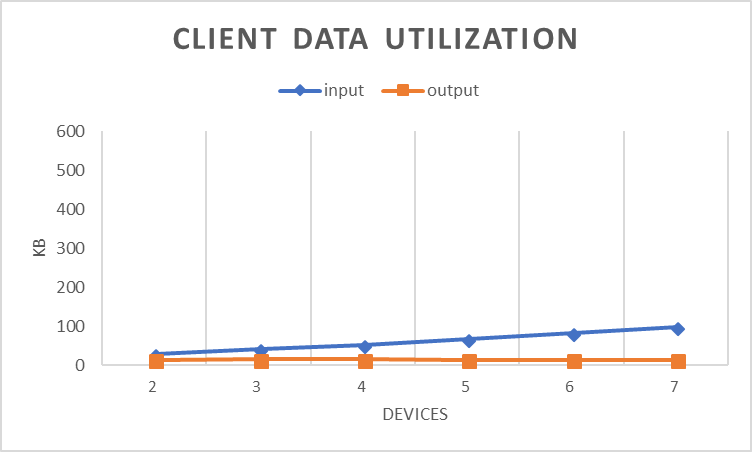
\includegraphics[scale=0.7]{client_data_utilization}
 \caption{Graph illustrating the input/output for a client}
 \label{fig:res:cdu}
\end{figure}

\begin{figure}[t]
 \centering
 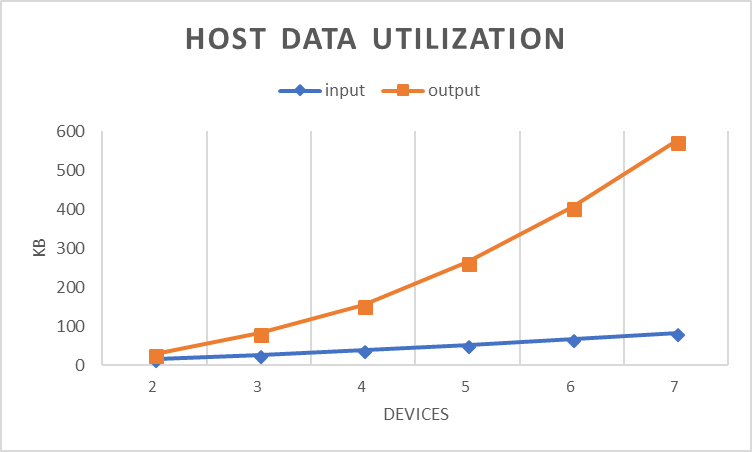
\includegraphics[scale=0.7]{host_data_utilization}
 \caption{Graph illustrating the input/output for a host}
 \label{fig:res:hdu}
\end{figure}

Analizing the graphs we obtained in Figure~\ref{fig:res:cdu} and 
Figure~\ref{fig:res:hdu}, we discovered that it follows a particular growth 
pattern based on the typology of the device: if the device is a host, we saw an 
exponential output growth and a small linear data increase in input relatively 
to the number of devices connected, instead when the device is a client we saw a 
linear increase of the data received based on the number of devices connected in 
a lobby. The output for the device client mode was not related to the number of 
the devices connected. To sum up the trend of data we collected satisfied our 
expectations.

In conclusion, the biggest data exchange is happening during the lobby 
formation. This is due the fact that profile pictures are exchanged and 
broadcated through all the peers. During the match, the traffic is very 
limited, because the transactions are relatively small, with an average size of 
only 500 Bytes. Thus, bluetooth particularly fit in this context, since most of 
the time the data sent between devices is quite small.
The only thing that surprised us was that Android is not able to support over 
seven simultaneous bluetooth connection. When we tried to connect eight devices 
we incurred in an Android bluetooth API crash.
